\documentclass[hyperref,UTF8]{article}
\usepackage{ctex}
\usepackage[margin=1in]{geometry}
\usepackage{booktabs}
\usepackage{bigstrut}
\usepackage{caption}
\usepackage{amsmath}
\usepackage{graphicx, subfig}
\usepackage{float}
\usepackage{colortbl}
\usepackage{listings}
\lstset{language=Matlab}%代码语言使用的是matlab
\lstset{breaklines}%自动将长的代码行换行排版
\lstset{extendedchars=false}%解决代码跨页时,章节标题,页眉等汉字不显示的问题

\usepackage[colorlinks,linkcolor=black]{hyperref}
\renewcommand\appendix{\setcounter{secnumdepth}{-2}}
\usepackage{multirow}
\usepackage{type1cm}
\usepackage{indentfirst}
\usepackage{setspace}
\usepackage{CJK}
\usepackage{ifthen}

\newcommand{\CJKfontsize}[4]{%
\fontsize{#1}{#2 plus#3 minus #4}\selectfont}
\geometry{a4paper,left=2cm,right=2cm,top=1cm,bottom=1cm}
\zihao{-4}
\geometry{a4paper,left=3.18cm,right=3.18cm,top=2.54cm,bottom=2.54cm}
\begin{document}
\thispagestyle{empty}
\tableofcontents
\thispagestyle{empty}
%\newpage\setcounter{page}{1}

\newpage\setcounter{page}{1}
\setlength{\baselineskip}{14pt}\zihao{-4}\songti{





\section{问题重述}
\subsection{问题背景}
近年来,经济结构战略性调整日益提上日程。从原来的采煤塌陷区,到国家级水利风景区,
徐州潘安湖风景区成为资源型地区经济向服务型地区经济转型发展的一个经典案例。
无论是作为潘安湖风景区的运营方、旅行团,还是风景区的游客,
是否有一个合理的风景区游览路线都是能否提供、获得良好出游体验的重要因素。
结合相关景点信息(见附表),建立相关数学模型,在规定的游览时间内,游历景区内的全部8个景点(
包括景石),在一定的顺序限制下,
为旅游爱好者或风景区运营方、旅行团设计合理的游览线路,完成以下几个问题。
\subsection{需要解决的问题}
\begin{enumerate}
\item 不考虑景点的游览和等待时间,1名游客从景石出发,所有景点至少游历一次,最终到达湿地商业街,至少需要经过多少距离。
建立数学模型,给出游览路线并计算最短游览长度。
\item 在前1问的基础上,考虑景点的游览时间,并假设游客平均速度为$V=2km/h$,
建立数学模型,设计游览线路,要求游客在12:00出发,
17:00前到达湿地商业街并在17:30离开的情况下,
他的总游览时间最长。给出相应的线路及游览时间。
\item 在前2问的基础上,1名游客改为3个旅行团,此时需要考虑等待时间,
建立数学模型,设计游览线路,要求3个旅行团的总游览时间最长。给出相应的路线及游览时间。
\item 在前3问的基础上,旅行团的步行速度可变,范围在$1km/h-3km/h$之间,但平均速度不能超过$2km/h$。
建立数学模型,设计游览线路,要求3个旅行团总游览时间最长、总等待时间最短。给出相应的线路及游览时间。
\item 事实上,实际生活中不同旅行团的出发时间不确定,每个景点的等待时间也不确定。考虑以上2个因素,
在前4问的基础上,建立数学模型,设计游览线路,使得多个旅行团的总游览时间长,总等待时间短。
\end{enumerate}



\section{模型假设}
\begin{enumerate}
\item 假设题目所给的数据真实可靠;
\item 对于森林小剧场,假设必须\textbf{恰好}整点、半点时才能进入;
\item 假设所有景点为质点,不考虑景点内的距离路程;
\item 所有需要等待的景点,假设上一组结束后,下一组立刻可以进入;
\item 假设游览过程中天气状况良好。
\end{enumerate}






\section{符号说明}
%下面是三线表
\begin{table}[htbp]
\centering
\caption{本文中所涉及的符号及说明}
%下一行有几个c就有几列
\begin{tabular}{cc}
\toprule
符号&意义\\
\midrule
$t_0$ & 游览时间\\
$t_1$ & 步行时间\\
$t_2$ & 等待时间\\
$d_k$ & 第k段路径的长度\\
$d_{ij}$ & 地点i到j的距离\\
$t_{ij}$ & 信息素浓度\\
$\Delta \psi_{xyz}$ & 方案x、y、z中同一景点游览时间的重合部分\\
$K_1$ & 步行时间影响因子\\
$ K_2$ & 等待时间影响因子\\
$M(w)$ & 可控性系数因子\\
\bottomrule
\end{tabular}
 \label{abs}
\end{table}











\section{问题分析}
\subsection{问题的重要性分析}
伴随着经济的发展,在满足温饱的前提下,人民越来越关注精神生活的提升,
旅游愈来愈成为人们喜闻乐见的休闲方式。

对于确定的目的地而言,
是否有一个合理的游览线路,直接影响着游客走的路程、花费的时间,
也间接影响着由此产生的花费及游览的心情。游览线路的合理程度影响着游客的游览体验。

无论是景区运营方、旅游团还是游客,游览行程的规划问题,都是无法避免的。
如何获得路程最短、花费时间最少的游览线路,这都需要合理的解决。

\subsection{相关文献综述}
关于游览路线的规划问题,在20世纪60年代的美国,就有科学家研究过。当时密执安大学的一位教授在对自然和人工自适应系统的研究过程中,模拟生物在自然环境中的遗传和进化过程形成了一种自适应全局优化概率搜索算法,即遗传算法。这在当时以至于延续到今日都受到了很大程度的认可。后续的关于这方面的问题还有模拟退火法、蚁群算法以及montocarlo算法等等。

\subsection{问题的思路分析}
关于徐州潘安湖风景区游览线路设计问题,本文进行了如下的分析:
\begin{enumerate}
\item 针对问题1,在不考虑等待时间及游览时间的前提下,
由于题目给出了2景点之间的最短距离,
我们认为不存在游历某个多余1次而时间或路程反而减少的情况,
此问转化为TSP类型问题。
\item 针对问题2,由于要考虑了游览时间,在各个景点中,需要着重考虑2个景点,
森林小剧场和游客服务中心。由于森林小剧场只在半点或整点开发,如何恰好到达该景点
以避免等待,成为一个重点。同时,注意到游客服务中心在16:00之后关闭,必须在
关闭前离开。而由于总的时间是一定的(12:00-17:30),只要路程花费的时间少,
游览的时间自然会多,因此本质上也可以为是问题1的延续
,只是需要考量森林小剧场和游客服务中心的变量。
\item 对于问题3而言,有1人变为3团,就需要考虑等待时间,相当于给问题2加了限制条件,
即在问题2的条件下,满足新的条件的路径时间规划设计。
\item 问题4则是问题3的更进一步,由于速度可变,考虑借由此条件尽可能消除等待时间,使花费的时间
尽可能多的在路程而不是等待上,在使得平均速度尽可能解决$2km/h$,即游览时间尽可能
化为总时间减去路程花费时间。
\item 对于问题五,引入修正变量,来尽可能地适应因旅行团出发时间不定、等待时间不定对模型
产生的影响。
\item 由于部分问题面临的选项过多,我们在进行模型设计的过程中,先行删除一些明显不合理的方案,
提高模型的时间效率。
\end{enumerate}



\section{模型的建立与求解}


\subsection{问题一}
针对问题一,我们需要求得从景石出发,到达湿地商业街,并且经过1到6所有景点至少1次的距离最短的路线。此问题,我们采用蚁群算法。

由于蚁群算法是求解从出发点又回到出发点的最短路径,我们需要对蚁群算法进行一定的改动。

\subsubsection{游览路线设计之路程最短(模型一)的建立}
蚁群模型如下

设蚂蚁的数量为$m$,地点的数量为$n$,地点$i$与地点$j$之间的距离为$d_{ij}$,$t$时刻地点$i$与地点$j$之间的信息素浓度为
$t_{ij}$ ,初始时刻,各个地点间连接路径上的信息素浓度相同,不妨记为$t_{ij}(0)=t_m$ ,
蚂蚁$k$根据各地点间连接路径上的信息素浓度,决定下一个要访问的城市,设$P(t)$表示$t$时刻,蚂蚁$k$从地点$i$到$j$的概率,其计算公式如下:
\begin{equation}\label{gongshi1}
P_{ij}^k=\left\{
\begin{array}{ccc}
 \frac{[t_{ij}(t)]^{\alpha}\bullet[{\eta}_{ij}(t)]^{\beta}}{{\sum_{s\in allow}}[t_{ij}(t)]^{\alpha}\bullet[{\eta}_{ij}(t)]^{\beta}  } & , & {s\in allow_k} \\
0 & , & {s \notin allow_k}
\end{array} \right.
\end{equation}

其中,${\eta}_{ij}(t)$为启发式函数,${\eta}_{ij}(t)=\frac{1}{d_{ij}}$,表示蚂蚁从地点$i$到地点$j$的期望程序。
$allow_k$表示蚂蚁待访问的地点的集合,开始时$allow_k$为其他$n-1$地点,随着时间的推进,其中的元素不断减少,直至为空,表示所有地点访问完,即遍历所有地点。而$t_{ij}(t)$则表示信息素情况,其更新公式为
\begin{equation}\label{gongshi3}
t_{ij}(t+1)=(1-\rho)t_{ij}(t)+\Delta t_{ij}(t)
\end{equation}
$\rho$ 为挥发系数(预设),$\Delta t_{ij}(t)$为$m$只蚂蚁均选择
下一地点后,所有选择有$i$到$j$的蚂蚁在该路径上遗留的信息素之和,其影响表达式为
\begin{equation}\label{gongshi4}
\Delta t_{ij}(t+1)=\sum_{k=1}^{m}\Delta t_{ij}^k(t)
\end{equation}
$\Delta t_{ij}^k(t)$表示第$k$只蚂蚁在路径$ij$上留下的信息素,可以认为
\begin{equation}\label{gongshi5}
\Delta t_{ij}^k(t)=\left\{
\begin{array}{ccc}
 {\frac{Q}{L^k(t)}} & , & {if\ k\ chooses\ i\ to\ j} \\
0 & , & others
\end{array} \right.
\end{equation}
$Q$为信息素强度(预设参数),$L^k(t)$则表示第$k$只蚂蚁在$t$时刻选择$i$到$j$后经过的所有地点路径长度,
为了找到最短路径,我们固定起点与终点,目标函数为
\begin{equation}\label{gongshi2}
f(w)=\sum_{i=1,j=1}^{n=6}d_{ij}+d_{0}+d_{7}
\end{equation}
其中,$w=(i_1,i_2,\cdots,i_6)$为景点$1,2,\cdots,6$的一个排列。
\subsubsection{游览路线设计之路程最短(模型一)的求解}
根据表\ref{xinxi1}所给出的数据画出图\ref{tu1},并标出每两点之间的距离。图中0为景石,1为游客服务中心,2为阳光草坪,3为森林小剧场,4为儿童科普体验区,5为儿童戏水场,6为湿地博物馆,7为湿地商业街。
\begin{figure}[htbp]
\centering
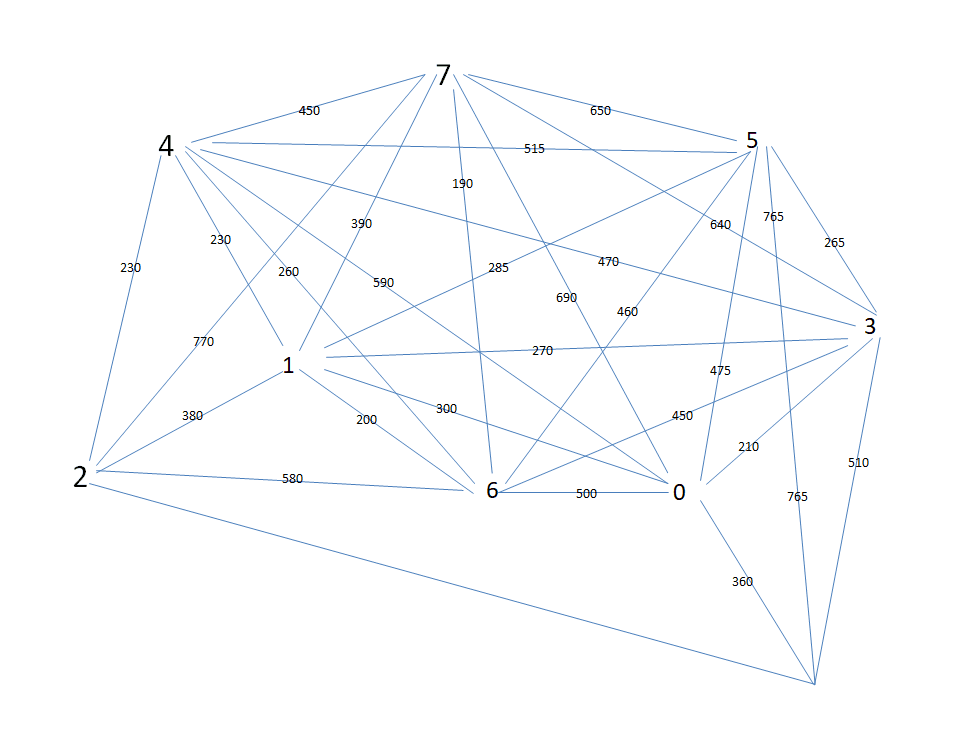
\includegraphics[width = 10cm]{20180501195944.png}
\caption{各景点间距离直观图}
\label{tu1}
\end{figure}

根据修改后的蚁群算法,利用MATLAB求得最短路线如表\ref{tab:addlabel1},最短的行程为$210+265+285+380+230+260+190=1820m$。


\begin{table}[htbp]
  \centering
  \caption{\textbf{第一问结果表格}}
    \begin{tabular}{|c|c|c|}
\hline
    出发景点  & 到达景点  & 步行距离(米) \\
\hline
    景石    & 森林小剧场 & 210 \\
\hline
    森林小剧场 & 儿童戏水场 & 265 \\
\hline
    儿童戏水场 & 游客服务中心 & 285 \\
\hline
    游客服务中心 & 阳光草坪  & 380 \\
\hline
    阳光草坪  & 儿童科普体验区 & 230 \\
\hline
    儿童科普体验区 & 湿地博物馆 & 260 \\
\hline
    湿地博物馆 & 湿地商业街 & 190 \\
\hline
\rowcolor[rgb]{ .553,  .702,  .886}  \multicolumn{2}{|c|}{总步行距离(最短路线距离)} & 1820 \\
\hline
\rowcolor[rgb]{ .553,  .702,  .886}  \multicolumn{2}{|c|}{最短路线(请用①~⑥序号标出)} & 景石$\to$ ③$\to$ ⑤$\to$ ①$\to$ ②$\to$ ④$\to$ ⑥$\to$⑦ \\
\hline
    \end{tabular}%
  \label{tab:addlabel1}%
\end{table}%


\subsection{问题二}
针对问题二,我们在问题一的基础上考虑游览时间最长,即需考虑步行时间及等待时间最少。
此时需注意各景点有其开放时间和游览时间(其中森林小剧场在半点和整点开放)。
\subsubsection{游览路线设计之游览时间最长(模型二)的准备}
设游览时间为$t_0$,步行时间为$t_1$,等待时间为$t_2$,则总的时间$t_0+t_1+t_2=330$(分钟)。

根据第一问,我们求得最路径的第一步为景石到森林小剧场,而其路程有$210m$,
速度为$2km/h$,需要$0.105$小时,即约为$6$分钟。那么则需在森林小剧场等待约$24$分钟$(t_2=24)$。
得到问题一所求得的方案$t_1+t_2=24+1.82/2*60=78.6min$。

由于这一过程经历了长时间的等待,
因此,我们需要判断是否存在其他更长的游览时间方案。
我们看到,由于其他景点的游览时间范围均较大,即无论第一步先选择去除森林小剧场外的任何景点,
都总可以找到合适的时间$t$,使得之后到达森林小剧场时可以实现恰好为开放时间,
因此,为了让森林小剧场的等待时间变短,我们使第一步不经过森林小剧场。
\subsubsection{游览路线设计之游览时间最长(模型二)的建立与求解}
不经过森林小剧场的目标函数改动为
\begin{equation}\label{wenti21}
f(w)=\sum_{i=1,j=1}^{n=6}d_{ij}'+d_{0}(w)+d_{7}
\end{equation}
其中,$d_0(w)\in \{d_{01},d_{02},d_{04},d_{05},d_{06}\}$,$d_{ij}'$为$d_{ij}$除去$d_0(w)$后的
对应数群。

利用MATLAB,此次使得第一步不经过森林小剧场,再根据蚁群算法求得最短路径,最长游览时间。由上文,
借由不同位置的$t$可达到同样的、恰好在森林小剧场开放时到达的效果,这里我们给出一种结果如表\ref{tab:addlabel2}。


% Table generated by Excel2LaTeX from sheet 'Sheet1'
\begin{table}[htbp]
  \centering
  \caption{\textbf{第二问结果表格(游览时间最长的路线信息)}}
    \begin{tabular}{|c|c|c|c|c|}
\hline
    \multicolumn{1}{|c|}{\multirow{2}[0]{*}{序号}} & \multicolumn{1}{c|}{\multirow{2}[0]{*}{景点名称}} & \multicolumn{1}{c|}{\multirow{2}[0]{*}{达到时间点}} & 游览时间  & \multicolumn{1}{c|}{\multirow{2}[0]{*}{离开时间点}} \\
          &       &       & (停留时间,单位分钟) &  \\
\hline
    1     & 景石    & \textbf{12:00:00} & 0.00  & \textbf{12:00:00} \\
\hline
    2     & 阳光草坪  & \textbf{12:10:48} & 60.00  & \textbf{13:10:48} \\
\hline
    3     & 儿童科普体验区 & \textbf{13:17:42} & 57.50  & \textbf{14:15:12} \\
\hline
    4     & 游客服务中心 & \textbf{14:21:54} & 30.00  & \textbf{14:51:54} \\
    \hline
    5     & 森林小剧场 & \textbf{15:00:00} & 30.00  & \textbf{15:30:00} \\
    \hline
    6     & 儿童戏水区 & \textbf{15:37:57} & 20.00  & \textbf{15:57:57}\\
    \hline
    7     & 湿地博物馆 & \textbf{16:11:45} & 30.00  & \textbf{16:41:45}\\
    \hline
    8     & 湿地商业街 & \textbf{16:47:27} & 42.55  & \textbf{17:30:00} \\
\hline
\multicolumn{5}{|c|}{\textbf{总的游览时间:269.85 分钟}}\\
\hline
\multicolumn{5}{|c|}{\textbf{总的步行时间:60.15  分钟}}\\ 
\hline
    \end{tabular}%
  \label{tab:addlabel2}%
\end{table}%

表中的消耗时间为$t_1+t_2=60.15+0=61.15$分钟,
小于由第一问得到的方案计算出的消耗时间$78.6$分钟,因此,模型二的结果是最长游览时间,为$269.85$分钟,游览线路更合适。

\subsection{问题三}
针对问题三,我们需要考虑由于不同旅行团到达同一景点后可能产生的等待时间,
目标是使得步行时间和等待时间的总和尽可能小。

此时同样需要考虑森林小剧场的整点半点开发特性以及游客服务中心的截止时间。
\subsubsection{游览路线设计之游览时间最长(模型三)的准备}
由于在问题三的情况下,游览时间是不确定的。而这不利于模型的量化分析,
因此我们直接使模型随机生成符合游览时间区间要求的时间值
,以足够的模拟值来弥补过多变量带来的不确定因素。同时,在不考虑等待因素的情况下,
随机生成游览线路。

为了简化模型的运算量,我们先行排除一些不合适方案:

考虑极端情况,如果三个旅行团一开始就前往同一个景点,必然伴随大量的等待时间。
因此显然一开始需要让3个旅行团前往不同的景点。、

而对于湿地商业街而言,其他地方到达湿地商业街的距离远大于湿地博物馆,
考虑到步行时间的影响。终点前一个位置定为6(湿地博物馆)。

\subsubsection{游览路线设计之游览时间最长(模型三)的建立与求解}
结合之前的准备,我们目前得到了足够多的、由随机的游览时间所形成的且排除一些错误方案后的游览方案。
直接进行等待时间的比较对于模型的运算量要求比较高,因此我们转而进行另一种方法:

比较所有生成的方案,计算相应的步行时间及方案间同一景点的重叠时间。显然,重叠时间越少,
可能面临的等待时间也就最少。重叠的部分越靠前,不可控的情况也越大;重叠的部分越靠后,不可控的情形越小。

结合以上的分析,我们给出新的消耗时间目标函数
\begin{equation}\label{wenti21}
f(w)=K_1\sum_{i=1,j=1}^{n=6}\frac{ d_{ij}}{V}+K_2\sum_{k=1}^{n=6}\Delta {\psi}_{xyz}\bullet M(w)
\end{equation}
其中,$K_1$,$K_2$为影响因子,分别调节步行时间与(可能的)等待时间对消耗时间的影响;
$\Delta {\psi}_{xyz}$为3个方案中,各个景点的重叠时间,当任意2个方案不存在重叠的时间时,$\Delta {\psi}_{xyz}=0$,
$M(w)$为可控性系数因子,当$\Delta {\psi}_{xyz}$代表的景点越靠前,该数越大。

利用MATLAB,结合消耗时间目标函数,根据蚁群算法求得最长游览时间,其结果如表\ref{tab:addlabel-1}、表\ref{tab:addlabel-2}、表\ref{tab:addlabel-3}所示。


\begin{table}[htbp]
  \centering
  \caption{\textbf{第三问结果表格-1}}
    \begin{tabular}{|c|c|c|c|}
    \hline
    \multicolumn{1}{|c|}{} & \multicolumn{3}{c|}{\textbf{第一旅游团}} \bigstrut\\
    \hline
    \multicolumn{1}{|c|}{} & 达到时间点 & \multicolumn{1}{p{4.055em}|}{游览时间(停留时间,单位分钟)} & \multicolumn{1}{p{4.055em}|}{离开时间点} \bigstrut\\
    \hline
    景石 & \multicolumn{1}{c|}{\textbf{12:00:00}} & \textbf{0} & \textbf{12:00:00} \bigstrut\\
    \hline
    游客服务中心 & \multicolumn{1}{c|}{\textbf{15:36:30}} & \textbf{10} & \textbf{15:46:30} \bigstrut\\
    \hline
    阳光草坪 & \multicolumn{1}{c|}{\textbf{12:10:48}} & \textbf{60} & \textbf{13:10:48} \bigstrut\\
    \hline
    森林小剧场 & \multicolumn{1}{c|}{\textbf{14:30:00}} & \textbf{30} & \textbf{15:00:00} \bigstrut\\
    \hline
    儿童科普体验区 & \multicolumn{1}{c|}{\textbf{13:17:42}} & \textbf{58.2} & \textbf{14:15:54} \bigstrut\\
    \hline
    儿童戏水场 & \multicolumn{1}{c|}{\textbf{15:07:57}} & \textbf{20} & \textbf{15:27:57} \bigstrut\\
    \hline
    湿地博物馆 & \multicolumn{1}{c|}{\textbf{15:52:30}} & \textbf{30} & \textbf{16:22:30} \bigstrut\\
    \hline
    湿地商业街 & \multicolumn{1}{c|}{\textbf{16:28:12}} & \textbf{61.8} & \textbf{17:30:00} \bigstrut\\
    \hline
    \textbf{总步行时间} & \multicolumn{3}{c|}{\textbf{60  分钟}} \bigstrut\\
    \hline
    \textbf{总游览时间} & \multicolumn{3}{c|}{\textbf{270 分钟}} \bigstrut\\
    \hline
    \textbf{总等待时间} & \multicolumn{3}{c|}{\textbf{0 分钟}} \bigstrut\\
    \hline
    \end{tabular}%
  \label{tab:addlabel-1}%
\end{table}%

\begin{table}[htbp]
  \centering
  \caption{\textbf{第三问结果表格-2}}
  \begin{tabular}{|c|c|c|c|}
    \hline
    \multicolumn{1}{|r|}{} & \multicolumn{3}{c|}{\textbf{第二旅游团}} \bigstrut\\
    \hline
    \multicolumn{1}{|r|}{} & 达到时间点 & \multicolumn{1}{p{4.055em}|}{游览时间(停留时间,单位分钟)} & \multicolumn{1}{p{4.055em}|}{离开时间点} \bigstrut\\
    \hline
    景石 & \multicolumn{1}{c|}{\textbf{12:00:00}} & \textbf{0} & \textbf{12:00:00} \bigstrut\\
    \hline
    游客服务中心 & \multicolumn{1}{c|}{\textbf{12:09:00}} & \textbf{30} & \textbf{12:39:00} \bigstrut\\
    \hline
    阳光草坪 & \multicolumn{1}{c|}{\textbf{14:45:18}} & \textbf{54} & \textbf{15:39:18} \bigstrut\\
    \hline
    森林小剧场 & \multicolumn{1}{c|}{\textbf{14:00:00}} & \textbf{30} & \textbf{14:30:00} \bigstrut\\
    \hline
    儿童科普体验区 & \multicolumn{1}{c|}{\textbf{15:46:12}} & \textbf{30} & \textbf{16:16:12} \bigstrut\\
    \hline
    儿童戏水场 & \multicolumn{1}{c|}{\textbf{12:47:33}} & \textbf{60} & \textbf{13:47:33} \bigstrut\\
    \hline
    湿地博物馆 & \multicolumn{1}{c|}{\textbf{16:24:00}} & \textbf{30.3} & \textbf{16:54:18} \bigstrut\\
    \hline
    湿地商业街 & \multicolumn{1}{c|}{\textbf{17:00:00}} & \textbf{30} & \textbf{17:30:00} \bigstrut\\
    \hline
    \textbf{总步行时间} & \multicolumn{3}{c|}{\textbf{61.2 分钟}} \bigstrut\\
    \hline
    \textbf{总游览时间} & \multicolumn{3}{c|}{\textbf{4.5 分钟}} \bigstrut\\
    \hline
    \textbf{总等待时间} & \multicolumn{3}{c|}{\textbf{264.5 分钟}} \bigstrut\\
    \hline
    \end{tabular}%
  \label{tab:addlabel-2}%
\end{table}%


\begin{table}[htbp]
  \centering
  \caption{\textbf{第三问结果表格-3}}
  \begin{tabular}{|c|c|c|c|}
    \hline
    \multicolumn{1}{|r|}{} & \multicolumn{3}{c|}{\textbf{第三旅游团}} \bigstrut\\
    \hline
    \multicolumn{1}{|r|}{} & 达到时间点 & \multicolumn{1}{p{4.055em}|}{游览时间(停留时间,单位分钟)} & \multicolumn{1}{p{4.055em}|}{离开时间点} \bigstrut\\
    \hline
    景石 & \multicolumn{1}{c|}{\textbf{12:00:00}} & \textbf{0} & \textbf{12:00:00} \bigstrut\\
    \hline
    游客服务中心 & \multicolumn{1}{c|}{\textbf{13:59:30}} & \textbf{10} & \textbf{14:09:30} \bigstrut\\
    \hline
    阳光草坪 & \multicolumn{1}{c|}{\textbf{14:26:24}} & \textbf{20} & \textbf{14:46:24} \bigstrut\\
    \hline
    森林小剧场 & \multicolumn{1}{c|}{\textbf{13:00:00}} & \textbf{30} & \textbf{13:30:00} \bigstrut\\
    \hline
    儿童科普体验区 & \multicolumn{1}{c|}{\textbf{14:26:24}} & \textbf{30} & \textbf{14:56:24} \bigstrut\\
    \hline
    儿童戏水场 & \multicolumn{1}{c|}{\textbf{12:14:15}} & \textbf{37.8} & \textbf{12:52:03} \bigstrut\\
    \hline
    湿地博物馆 & \multicolumn{1}{c|}{\textbf{15:04:12}} & \textbf{30} & \textbf{15:34:12} \bigstrut\\
    \hline
    湿地商业街 & \multicolumn{1}{c|}{\textbf{15:39:54}} & \textbf{110.1} & \textbf{17:30:00} \bigstrut\\
    \hline
    \textbf{总步行时间} & \multicolumn{3}{c|}{\textbf{62.1 分钟}} \bigstrut\\
    \hline
    \textbf{总游览时间} & \multicolumn{3}{c|}{\textbf{267.9 分钟}} \bigstrut\\
    \hline
    \textbf{总等待时间} & \multicolumn{3}{c|}{\textbf{0  分钟}} \bigstrut\\
    \hline
    \end{tabular}%
  \label{tab:addlabel-3}%
\end{table}%

从中我们得到结论,3个旅行团的总最长游览时间为$t_0=270+264.5+267.9=802.2$分钟,步行时间为$t_1=60+61.2+62.1=183.3$分钟,
等待时间为$t_2=0+4.5+0=4.5$分钟。

\subsection{问题四}
\subsubsection{游览路线设计之游览时间最长(模型四)的建立}
针对问题四,由于速度可变,游览路线的设计变得更加复杂。与问题三类似的,
我们不直接计算因速度变化而影响的等待时间,而是随机生成范围在$1km/h-3km/h$的、平均值不超过$2km/h$的速度值,
同样借助大量的模拟来减少变量过多带来的多情况讨论。

此时消耗时间函数须修改为
\begin{equation}\label{wenti41}
f(w)=K_1\sum_{i=1,j=1}^{n=6}\frac{d_{ij}}{V_{ij}}+K_2\sum_{k=1}^{n=6}\Delta {\psi}_{xyz}\bullet M(w)
\end{equation}
其中,$V_{ij}$为各景点间步行的速度,满足
\begin{equation}\label{wenti21}
\left\{
\begin{array}{c}
1km/h \le V_{ij} \le 3km/h\\
E(V)\le 2km/h
\end{array} \right.
\end{equation}
\subsubsection{游览路线设计之游览时间最长(模型四)的求解}
利用MATLAB,结合消耗时间函数,根据蚁群算法求得最长游览时间,其结果如表\ref{tab:addlabel+1}、表\ref{tab:addlabel+2}、表\ref{tab:addlabel+3}所示。

\begin{table}[htbp]
  \centering
  \caption{\textbf{第四问结果表格-1}}
    \begin{tabular}{|c|c|c|c|c|}
    \hline
       & \multicolumn{4}{c|}{\textbf{第一旅游团}} \bigstrut\\
    \hline
       & \multicolumn{1}{p{4.055em}|}{达到时间点} & \multicolumn{1}{p{4.055em}|}{游览时间(停留时间,单位分钟)} & \multicolumn{1}{p{4.055em}|}{离开时间点} & \multicolumn{1}{p{4.055em}|}{达到下一个景点的步行速度} \bigstrut\\
    \hline
    \multicolumn{1}{|p{4.055em}|}{景石} & \textbf{12:00:00} & \textbf{0} & \textbf{12:00:00} & \multicolumn{1}{p{4.055em}|}{\textbf{2km/h}} \bigstrut\\
    \hline
    \multicolumn{1}{|p{4.055em}|}{游客服务中心} & \textbf{15:36:30} & \textbf{10} & \textbf{15:46:30} & \multicolumn{1}{p{4.055em}|}{\textbf{2km/h}} \bigstrut\\
    \hline
    \multicolumn{1}{|p{4.055em}|}{阳光草坪} & \textbf{12:10:48} & \textbf{60} & \textbf{13:10:48} & \multicolumn{1}{p{4.055em}|}{\textbf{2km/h}} \bigstrut\\
    \hline
    \multicolumn{1}{|p{4.055em}|}{森林小剧场} & \textbf{14:30:00} & \textbf{30} & \textbf{15:00:00} & \multicolumn{1}{p{4.055em}|}{\textbf{2km/h}} \bigstrut\\
    \hline
    \multicolumn{1}{|p{4.055em}|}{儿童科普体验区} & \textbf{13:17:42} & \textbf{58.2} & \textbf{14:15:54} & \multicolumn{1}{p{4.055em}|}{\textbf{2km/h}} \bigstrut\\
    \hline
    \multicolumn{1}{|p{4.055em}|}{儿童戏水场} & \textbf{15:07:57} & \textbf{20} & \textbf{15:27:57} & \multicolumn{1}{p{4.055em}|}{\textbf{2km/h}} \bigstrut\\
    \hline
    \multicolumn{1}{|p{4.055em}|}{湿地博物馆} & \textbf{15:52:30} & \textbf{30} & \textbf{16:22:30} & \multicolumn{1}{p{4.055em}|}{\textbf{2km/h}} \bigstrut\\
    \hline
    \multicolumn{1}{|p{4.055em}|}{湿地商业街} & \textbf{16:28:12} & \textbf{61.8} & \textbf{17:30:00} & \textbf{0} \bigstrut\\
    \hline
    \multicolumn{1}{|p{4.055em}|}{\textbf{总步行时间}} & \multicolumn{4}{c|}{\textbf{60 分钟}} \bigstrut\\
    \hline
    \multicolumn{1}{|p{4.055em}|}{\textbf{总游览时间}} & \multicolumn{4}{c|}{\textbf{270 分钟}} \bigstrut\\
    \hline
    \multicolumn{1}{|p{4.055em}|}{\textbf{总等待时间}} & \multicolumn{4}{c|}{\textbf{0 分钟}} \bigstrut\\
    \hline
    \multicolumn{1}{|c|}{\multirow{2}[2]{*}{\textbf{平均速度}}} & \multicolumn{4}{c|}{\multirow{2}[2]{*}{ 2Km/h}} \bigstrut[t]\\
       & \multicolumn{4}{c|}{} \bigstrut[b]\\
    \hline
    \end{tabular}%
  \label{tab:addlabel+1}%
\end{table}%
% Table generated by Excel2LaTeX from sheet 'Sheet4'
\begin{table}[htbp]
  \centering
  \caption{\textbf{第四问结果表格-2}}
    \begin{tabular}{|c|c|c|c|c|}
    \hline
       & \multicolumn{4}{c|}{\textbf{第二旅游团}} \bigstrut\\
    \hline
       & \multicolumn{1}{p{4.055em}|}{达到时间点} & \multicolumn{1}{p{4.055em}|}{游览时间(停留时间,单位分钟)} & \multicolumn{1}{p{4.055em}|}{离开时间点} & \multicolumn{1}{p{4.055em}|}{达到下一个景点的步行速度} \bigstrut\\
    \hline
    \multicolumn{1}{|p{4.055em}|}{景石} & \textbf{12:00:00} & \textbf{0} & \textbf{12:00:00} & \multicolumn{1}{p{4.055em}|}{\textbf{2km/h}} \bigstrut\\
    \hline
    \multicolumn{1}{|p{4.055em}|}{游客服务中心} & \textbf{12:09:00} & \textbf{30} & \textbf{12:39:00} & \multicolumn{1}{p{4.055em}|}{\textbf{2km/h}} \bigstrut\\
    \hline
    \multicolumn{1}{|p{4.055em}|}{阳光草坪} & \textbf{14:45:18} & \textbf{54} & \textbf{15:39:18} & \multicolumn{1}{p{4.055em}|}{\textbf{2.45km/h}} \bigstrut\\
    \hline
    \multicolumn{1}{|p{4.055em}|}{森林小剧场} & \textbf{14:00:00} & \textbf{30} & \textbf{14:30:00} & \multicolumn{1}{p{4.055em}|}{\textbf{2km/h}} \bigstrut\\
    \hline
    \multicolumn{1}{|p{4.055em}|}{儿童科普体验区} & \textbf{15:44:56} & \textbf{34.5} & \textbf{16:19:26} & \multicolumn{1}{p{4.055em}|}{\textbf{2.4km/h}} \bigstrut\\
    \hline
    \multicolumn{1}{|p{4.055em}|}{儿童戏水场} & \textbf{12:47:33} & \textbf{60} & \textbf{13:47:33} & \multicolumn{1}{p{4.055em}|}{\textbf{1.28km/h}} \bigstrut\\
    \hline
    \multicolumn{1}{|p{4.055em}|}{湿地博物馆} & \textbf{15:44:56} & \textbf{30.3} & \textbf{16:15:14} & \multicolumn{1}{p{4.055em}|}{\textbf{3km/h}} \bigstrut\\
    \hline
    \multicolumn{1}{|p{4.055em}|}{湿地商业街} & \textbf{17:00:00} & \textbf{30} & \textbf{17:30:00} & \textbf{0} \bigstrut\\
    \hline
    \multicolumn{1}{|p{4.055em}|}{\textbf{总步行时间}} & \multicolumn{4}{c|}{\textbf{61.2 分钟}} \bigstrut\\
    \hline
    \multicolumn{1}{|p{4.055em}|}{\textbf{总游览时间}} & \multicolumn{4}{c|}{\textbf{268.8  分钟}} \bigstrut\\
    \hline
    \multicolumn{1}{|p{4.055em}|}{\textbf{总等待时间}} & \multicolumn{4}{c|}{\textbf{0分钟}} \bigstrut\\
    \hline
    \multicolumn{1}{|c|}{\multirow{2}[2]{*}{\textbf{平均速度}}} & \multicolumn{4}{c|}{\multirow{2}[2]{*}{ 2Km/h}} \bigstrut[t]\\
       & \multicolumn{4}{c|}{} \bigstrut[b]\\
    \hline
    \end{tabular}%
  \label{tab:addlabel+2}%
\end{table}%

\begin{table}[htbp]
  \centering
  \caption{\textbf{第四问结果表格-3}}
    \begin{tabular}{|c|c|c|c|c|}
    \hline
       & \multicolumn{4}{c|}{\textbf{第三旅游团}} \bigstrut\\
    \hline
       & \multicolumn{1}{p{4.055em}|}{达到时间点} & \multicolumn{1}{p{4.055em}|}{游览时间(停留时间,单位分钟)} & \multicolumn{1}{p{4.055em}|}{离开时间点} & \multicolumn{1}{p{4.055em}|}{达到下一个景点的步行速度} \bigstrut\\
    \hline
    \multicolumn{1}{|p{4.055em}|}{景石} & \textbf{12:00:00} & \textbf{0} & \textbf{12:00:00} & \multicolumn{1}{p{4.055em}|}{\textbf{2km/h}} \bigstrut\\
    \hline
    \multicolumn{1}{|p{4.055em}|}{游客服务中心} & \textbf{13:59:30} & \textbf{10} & \textbf{14:09:30} & \multicolumn{1}{p{4.055em}|}{\textbf{2km/h}} \bigstrut\\
    \hline
    \multicolumn{1}{|p{4.055em}|}{阳光草坪} & \textbf{14:26:24} & \textbf{20} & \textbf{14:46:24} & \multicolumn{1}{p{4.055em}|}{\textbf{2km/h}} \bigstrut\\
    \hline
    \multicolumn{1}{|p{4.055em}|}{森林小剧场} & \textbf{13:00:00} & \textbf{30} & \textbf{13:30:00} & \multicolumn{1}{p{4.055em}|}{\textbf{2km/h}} \bigstrut\\
    \hline
    \multicolumn{1}{|p{4.055em}|}{儿童科普体验区} & \textbf{14:26:24} & \textbf{30} & \textbf{14:56:24} & \multicolumn{1}{p{4.055em}|}{\textbf{2km/h}} \bigstrut\\
    \hline
    \multicolumn{1}{|p{4.055em}|}{儿童戏水场} & \textbf{12:14:15} & \textbf{37.8} & \textbf{12:52:03} & \multicolumn{1}{p{4.055em}|}{\textbf{2km/h}} \bigstrut\\
    \hline
    \multicolumn{1}{|p{4.055em}|}{湿地博物馆} & \textbf{15:04:12} & \textbf{30} & \textbf{15:34:12} & \multicolumn{1}{p{4.055em}|}{\textbf{2km/h}} \bigstrut\\
    \hline
    \multicolumn{1}{|p{4.055em}|}{湿地商业街} & \textbf{15:39:54} & \textbf{110.1} & \textbf{17:30:00} & \textbf{0} \bigstrut\\
    \hline
    \multicolumn{1}{|p{4.055em}|}{\textbf{总步行时间}} & \multicolumn{4}{c|}{\textbf{62.1分钟}} \bigstrut\\
    \hline
    \multicolumn{1}{|p{4.055em}|}{\textbf{总游览时间}} & \multicolumn{4}{c|}{\textbf{267.9 分钟}} \bigstrut\\
    \hline
    \multicolumn{1}{|p{4.055em}|}{\textbf{总等待时间}} & \multicolumn{4}{c|}{\textbf{0 分钟}} \bigstrut\\
    \hline
    \multicolumn{1}{|c|}{\multirow{2}[2]{*}{\textbf{平均速度}}} & \multicolumn{4}{c|}{\multirow{2}[2]{*}{ 2Km/h}} \bigstrut[t]\\
       & \multicolumn{4}{c|}{} \bigstrut[b]\\
    \hline
    \end{tabular}%
  \label{tab:addlabel+3}%
\end{table}%

从中我们得到结论,在步行速度较为灵活的情况下,等待时间可以被消除,
3个旅行团的总最长游览时间为$t_0=270+268.8+267.9=806.7$分钟,步行时间为$t_1=60+61.2+62.1=183.3$分钟。

\subsection{问题五}
\subsubsection{游览路线设计之不同时间出发的游览时间最长(模型五-1)的建立}
为了解决旅行团出发时间不相等的问题,我们只需要在原先的模型基础上,
改变不同旅行团的出发时间,然后通过模型得到其游览路线以及到达每个景点的时间,
进而比较所有生成的方案,计算相应的步行时间及方案间同一景点的重叠时间。

约束函数追加新的条件,变更为
\begin{equation}\label{wenti51}
f(w)=K_1\sum_{i=1,j=1}^{n=6}\frac{ d_{ij}}{V_{ij}}+K_2\sum_{k=1}^{n=6}\Delta {\psi}_{xyz}\bullet M(w)+N(w)
\end{equation}
通过增加出发时间差异触发因子$N(w)$,来实现对不同出发时间的旅行团线路设计。

根据先前的模型以及经验,显然,重叠时间越少,可能面临的等待时间也就最少。

为了检验这个模型,我们随机生成了多个不同出发时间的旅行团,在进行模型分析后,发现得到的路线均得到了不同程度的改变。
我们发现后面加入的旅行团的出发时间差距越大,对原最佳路线的影响就会越少。
\subsubsection{游览路线设计之等待时间未定的游览时间最长(模型五-2)的建立}
等待时间的差异是指在原来的问题基础上,考虑到旅游设施短时间的维护和清理,
或者受到散客客流的影响造成的等待时间。

旅游设施短时间的维护和清理,
会导致维护时间抵达该景点的旅游团必须要等待,
散客客流较大的景点也会导致旅游团的等待。

我们采用的解决方法是将这些问题造成的等待时间转化为一个旅游团的游览问题。
在额外的等待事件发生时,可视为有一个旅游团在这段时间到达该景点并进行游览,
其余旅游团到达该地点时需要等待。
这就将额外事件触发的等待时间转化为多一个旅游团的问题,
再带入相关模型(\ref{wenti41})求解可得最佳方案。




\section{模型检验与分析}
\subsection{假设的合理性分析}
\begin{enumerate}
\item 假设1使每两个地点间的距离与相关时间真实可靠;
\item 假设2简化了对于森林小剧场的分析,排除了时间区间带来的影响;
\item 假设3排除了游览景点时产生的路程对游览路线规划带来的影响;
\item 假设4排除了进出带来的等待时间差异问题;
\item 假设5排除了一些特殊情况对路径规划的影响。
\end{enumerate}
\subsection{可靠性分析(给出模型的使用范围)}
本文以蚁群模型为基础,针对不同的问题,引入不同的约束函数,以达到最短路径或
最长时间停留各个目的地的最优算法模型。借助重叠比较的方法,完成多线路的方案设计。

此模型经过合理改进之后可以适用于各种旅游路径规划,甚至是多线并行的现代物流配送方案设计,
及最优方案设计,最优时间方案设计等各种问题,具有相当广泛的适用范围。

\subsection{模型的合理性分析}
本文建立的模型充分考虑到了各种原始条件的相互制约关系,通过假设,
考虑原始数据的真实性与合理性,即原始条件以及数据的合理性。

同时,模型利用蚁群算法,根据不同问题,有针对性的引入目标函数,达到最优路径规划设计,
即模型设计中算法过程以及求解过程的合理,可信。

最终的结果进行确认,借助迭代的方式得出结果,即结果的合理性。




\section{模型的评价与推广}
\subsection{模型的优缺点分析}
\subsubsection{模型的优点}
\begin{enumerate}
\item 通过合理且适当的假设,首先去除了一些特殊因素的干扰,提升了计算结果的可靠性;
\item 采用蚁群算法,搜索过程采用分布式计算方式,多个个体同时进行并行计算,大大提高了算法的计算能力和运行效率。
启发式的概率搜索方式不容易陷入局部最优,易于寻找到全局最优解。;
\item 针对不同的问题,引入不同的目标函数,对问题的适应性较好;
\item 考虑到了旅游团出行时间、等待时间等多种因素,符合实际情况。
\end{enumerate}
\subsubsection{模型的缺点}
\begin{enumerate}
\item 本模型将所有景点视为质点,可能存在模拟计算路线具体只不完全精确的情况;
\item 虽然引入了约束函数,并且排除了一部分选项。但需要考虑的情况仍然很多,花费的时间可能较多。
\end{enumerate}
\subsection{模型的优化}
\begin{enumerate}
\item 可以对随机生成的速度、时间也引入诱导因子$s_i,r_i$,形成三维蚁群,减少迭代次数。
\item 考虑到人的精力对步行速度的影响(时间越长,速度会一定程度上减慢),可以引入速度变更因子$v_i$。
\end{enumerate}

\subsection{模型的应用邻域及推广}
\begin{enumerate}
\item 本模型基于蚁群模型,可以适用于各种旅游路径的规划。
\item 对于物流行业,也可应用:多线并行的现代物流配送方案设计,
及最优方案设计,最优时间方案设计等各种问题。
\end{enumerate}

\begin{thebibliography}{99}
\addcontentsline{toc}{section}{参考文献}
\bibitem{1}谭阳. 求解广义旅行商问题的若干进化算法研究[D].华南理工大学,2013.
\bibitem{2}http://www.cnblogs.com/biaoyu/archive/2012/09/26/2704456.html
\bibitem{3}https://blog.csdn.net/lanjiangzhou/article/details/9097585
\bibitem{4}https://blog.csdn.net/specter11235/article/details/68947006
\bibitem{5}https://blog.csdn.net/xyisv/article/details/79184815
\end{thebibliography}
}
\appendix
\section{附录}
\subsection{徐州潘安湖风景区景点相关信息}
徐州潘安湖风景区景点相关信息分别见表\ref{xinxi1}与表\ref{xinxi2}
\begin{table}[htbp]
  \centering
  \caption{\textbf{景点之间的最短步行距离(单位:米)}}\label{xinxi1}%
    \begin{tabular}{|p{4.555em}|c|c|c|c|c|c|c|c|}
    \hline
    \multicolumn{1}{|p{3.055em}|}{} & \multicolumn{1}{p{3.055em}|}{景石} & \multicolumn{1}{p{3.055em}|}{游客服务中心} & \multicolumn{1}{p{3.055em}|}{阳光草坪} & \multicolumn{1}{p{3.055em}|}{森林小剧场} & \multicolumn{1}{p{3.055em}|}{儿童科普体验区} & \multicolumn{1}{p{3.055em}|}{儿童戏水场} & \multicolumn{1}{p{3.055em}|}{湿地博物馆} & \multicolumn{1}{p{4.055em}|}{湿地商业街} \bigstrut\\
    \hline
    景石    & 0     & 300   & 360   & 210   & 590   & 475   & 500   & 690 \bigstrut\\
    \hline
    游客服务中心 & 300   & 0     & 380   & 270   & 230   & 285   & 200   & 390 \bigstrut\\
    \hline
    阳光草坪  & 360   & 380   & 0     & 510   & 230   & 765   & 580   & 770 \bigstrut\\
    \hline
    森林小剧场 & 210   & 270   & 510   & 0     & 470   & 265   & 450   & 640 \bigstrut\\
    \hline
    儿童科普体验区 & 590   & 230   & 230   & 470   & 0     & 515   & 260   & 450 \bigstrut\\
    \hline
    儿童戏水场 & 475   & 285   & 765   & 265   & 515   & 0     & 460   & 650 \bigstrut\\
    \hline
    湿地博物馆 & 500   & 200   & 580   & 450   & 260   & 460   & 0     & 190 \bigstrut\\
    \hline
    湿地商业街 & 690   & 390   & 760   & 640   & 450   & 650   & 190   & 0 \bigstrut\\
    \hline
    \end{tabular}%

\end{table}%


\begin{table}[htbp]
  \centering
  \caption{\textbf{各景点游览时间}}\label{xinxi2}%
    \begin{tabular}{|p{7.61em}|p{5.055em}|p{24.165em}|}
    \hline
                 时间 & \multirow{2}[2]{*}{游览时间} & \multirow{2}[2]{*}{开放时间} \bigstrut[t]\\
    景点    & \multicolumn{1}{r|}{} & \multicolumn{1}{r|}{} \bigstrut[b]\\
    \hline
    游客服务中心 & 10-30分钟 & 9:00-16:00 \bigstrut\\
    \hline
    阳光草坪  & 20-60分钟 & 9:00-17:00 \bigstrut\\
    \hline
    森林小剧场 & 30分钟  & 9:00, 9:30, 10:00, 10:30, 11:00, 11:30, 12:00, 12:30, 13:00, 13:30, 14:00, 14:30, 15:00, 15:30, 16:00, 16:30, 17:00 (半点和整点开放) \bigstrut\\
    \hline
    儿童科普体验区 & 30-60分钟 & 9:00-17:00 \bigstrut\\
    \hline
    儿童戏水场 & 20-60分钟 & 9:00-17:00 \bigstrut\\
    \hline
    湿地博物馆 & 30-60分钟 & 9:00-17:00 \bigstrut\\
    \hline
    湿地商业街 & 30分钟以上 & 9:00-21:30 \bigstrut\\
    \hline
    \end{tabular}%
  
\end{table}%

\subsection{Matlab模型源代码}
\subsubsection{模型一、二}
\begin{lstlisting}
%蚁群算法(多人TSP)
%%数据准备
clear;
clc;
t0=clock;%程序开始的计时
%%初始化参数
a=zeros(8,8);
n=6;
for i=1:8
    for j=1:8
        a(i,j)=1e-4;%设定的对角矩阵修正值,防止对角出现0
    end
end
a(1,2)=380; a(1,3)=270; a(1,4)=230; a(1,5)=285; a(1,6)=200; a(1,7)=390; a(1,8)=300; 
a(2,3)=510; a(2,4)=230; a(2,5)=765; a(2,6)=580; a(2,7)=770; a(2,8)=360; 
a(3,4)=470; a(3,5)=265; a(3,6)=450; a(3,7)=640; a(3,8)=210;    
a(4,5)=515; a(4,6)=260; a(4,7)=450; a(4,8)=590;  
a(5,6)=460; a(5,7)=650; a(5,8)=475;
a(6,7)=190; a(6,8)=500;
a(2,1)=380; a(3,1)=270; a(4,1)=230; a(5,1)=285; a(6,1)=200; a(7,1)=390;
a(3,2)=510; a(4,2)=230; a(5,2)=765; a(6,2)=580; a(7,2)=770; 
a(4,3)=470; a(5,3)=265; a(6,3)=450; a(7,3)=640;     
a(5,4)=515; a(6,4)=260; a(7,4)=450;   
a(6,5)=460; a(7,5)=650; 
a(7,6)=190;
B = a(1:6, 1:6);
m=10;           %蚂蚁数量
alpha=1;        %信息素重要程度因子
beta=5;         %启发函数重要程度因子
vol=0.2;          %信息素挥发因子
Q=10;           %常系数
Heu_F=1./B;    %启发函数
Tau=ones(n,n);     %信息素矩阵
Table=zeros(m,n);   %路径记录表
iter=1;                     %迭代次数初值
iter_max=100;           %最大迭代系数
Route_best=zeros(iter_max,n);       %各代最佳路径
Length_best=zeros(iter_max,1);         %各代最佳路径的长度
Length_ave=zeros(iter_max,1);           %各代路径的平均长度
Limit_iter=0;                               %程序收敛时迭代次数
%%迭代法找最佳路径
while iter<=iter_max            %随机产生各个蚂蚁的起点城市
    start=zeros(m,1);
   % for i=1:m
    %    temp=randperm(n);
     %   start(i)=7;
      %  Table(i,1)=7;           %构筑解空间
    %end
i=1;
while i<11
     temp=randperm(n);
     if temp(1)~=3
        start(i)=temp(1);
        i=i+1;
     end
end
    Table(:,1)=start;
    citys_index=1:n;           %逐个蚂蚁的路径选择
    for i=1:m                       %逐个城市路径选择
        for j=2:n
            tabu=Table(i,1:(j-1));      %已访问的城市集合(禁忌表)
            allow_index=~ismember(citys_index,tabu);    %判断变量是否出现,即是否访问过,返回0-1矩阵
            allow=citys_index(allow_index);                        %待访问的城市集合
            P=allow;                                                            %计算城市间的转移概率
            for k=1:length(allow)
                P(k)=Tau(tabu(end),allow(k))^alpha*Heu_F(tabu(end),allow(k))^beta;
            end
            P=P/sum(P);                                                        %轮盘赌法(随机且不重复)选择下一个访问城市
            Pc=cumsum(P);                                                   %求累加和
            target_index=find(Pc>=rand);                    
            target=allow(target_index(1));
            Table(i,j)=target;
        end
    end                                                                         %计算各个蚂蚁的路径距离
    Length=zeros(m,1);
    for i=1:m
        Route=Table(i,:);
        for j=1:(n-1)
            Length(i)=Length(i)+B(Route(j),Route(j+1));
        end
       % Length(i)=Length(i)+a(Route(n),8);
       Length(i)=Length(i)+a(Route(1),8)+a(Route(n),7);
    end                                                                     %计算最短路径距离及平均距离
    if iter==1
        [min_Length,min_index]=min(Length);
        Length_best(iter)=min_Length;
        Length_ave(iter)=mean(Length);
        Route_best(iter,:)=Table(min_index,:);
        Limit_iter=1;
    else 
        [min_Length,min_index]=min(Length);
        Length_best(iter)=min(Length_best(iter-1),min_Length);
        Length_ave(iter)=mean(Length);
        if Length_best(iter)==min(Length)
            Route_best(iter,:)=Table(min_index,:);
            Limit_iter=iter;
        else
            Route_best(iter,:)=Route_best((iter-1),:);
        end
    end                                                                         %更新信息素
    Delta_Tau=zeros(n,n);                                               %逐个蚂蚁计算
    for i=1:m                                                                   %逐个城市计算
        for j=1:(n-1)
            Delta_Tau(Table(i,j),Table(i,j+1))=Delta_Tau(Table(i,j),Table(i,j+1))+Q/Length(i);
        end
        Delta_Tau(Table(i,n),Table(i,1))=Delta_Tau(Table(i,n),Table(i,1))+Q/Length(i);
    end
    Tau=(1-vol)*Tau+Delta_Tau;                                              %迭代次数+1,清空路径记录表
    iter=iter+1;
    Table=zeros(m,n);
end
%%输出结果
[Shortest_Length,index]=min(Length_best);
Shortest_Route=Route_best(index,:);
Time_Cost=etime(clock,t0);
disp(['最短距离:' num2str(Shortest_Length)]);
disp(['最短路径:' num2str([8 Shortest_Route 7])]);
disp(['收敛迭代次数:' num2str(Limit_iter)]);
disp(['程序执行时间:' num2str(Time_Cost) '秒']);
%%绘图表示
figure(1)
plot([citys(Shortest_Route,1);citys(Shortest_Route(1),1)],[citys(Shortest_Route,2);citys(Shortest_Route(1),2)],'o-');
grid on
for i=1:size(citys,1)
    text(citys(i,1),citys(i,2),['    ' num2str(i)]);
end
text(citys(Shortest_Route(1),1),citys(Shortest_Route(1),2),'    起点');
text(citys(Shortest_Route(end),1),citys(Shortest_Route(end),2),'    终点');
xlabel('城市位置横坐标')
ylabel('城市位置纵坐标')
title(['ACA最优化路径(最短距离:‘ num2str(Shortest_Length)’)'])
figure(2)
plot(1:iter_max,Length_best,'b')
legend('最短距离')
xlabel('迭代次数')
ylabel('距离')
title('算法收敛轨迹')
\end{lstlisting}
\subsubsection{模型三、四、五}
\begin{lstlisting}
%蚁群算法改进:以三只蚂蚁为一组
%%数据准备
clear;
clc;
t0=clock;%程序开始的计时
a=zeros(8,8);
n=5;
for i=1:8
    for j=1:8
        a(i,j)=1e-4;%设定的对角矩阵修正值,防止对角出现0
    end
end
a(1,2)=380; a(1,3)=270; a(1,4)=230; a(1,5)=285; a(1,6)=200; a(1,7)=390; a(1,8)=300; 
a(2,3)=510; a(2,4)=230; a(2,5)=765; a(2,6)=580; a(2,7)=770; a(2,8)=360; 
a(3,4)=470; a(3,5)=265; a(3,6)=450; a(3,7)=640; a(3,8)=210;    
a(4,5)=515; a(4,6)=260; a(4,7)=450; a(4,8)=590;  
a(5,6)=460; a(5,7)=650; a(5,8)=475;
a(6,7)=190; a(6,8)=500;
a(2,1)=380; a(3,1)=270; a(4,1)=230; a(5,1)=285; a(6,1)=200; a(7,1)=390;
a(3,2)=510; a(4,2)=230; a(5,2)=765; a(6,2)=580; a(7,2)=770; 
a(4,3)=470; a(5,3)=265; a(6,3)=450; a(7,3)=640;     
a(5,4)=515; a(6,4)=260; a(7,4)=450;   
a(6,5)=460; a(7,5)=650; 
a(7,6)=190;
B = a(1:7, [1,2,3,4,5,6,8]);%保存除最后一个点的路线点
m=20;           %蚂蚁数量
alpha=1;        %信息素重要程度因子
beta=5;         %启发函数重要程度因子
vol=0.2;          %信息素挥发因子
Q=10;           %常系数
Heu_F=1./B;    %启发函数
Tau=ones(n,n);     %信息素矩阵
Table=zeros(m,n);   %路径记录表
iter=1;                     %迭代次数初值
iter_max=100000;           %最大迭代系数
Route_best=zeros(iter_max,n);       %各代最佳路径
Length_best=zeros(iter_max,1);         %各代最佳路径的长度
Length_ave=zeros(iter_max,1);           %各代路径的平均长度
Limit_iter=0;                               %程序收敛时迭代次数

Tau1=ones(n,n);     %信息素矩阵
Table1=zeros(m,n);   %路径记录表
iter1=1;                     %迭代次数初值
iter_max1=100;           %最大迭代系数
Route_best1=zeros(iter_max1,n);       %各代最佳路径
Length_best1=zeros(iter_max1,1);         %各代最佳路径的长度
Length_ave1=zeros(iter_max1,1);           %各代路径的平均长度
Limit_iter1=0;                               %程序收敛时迭代次数

Tau2=ones(n,n);     %信息素矩阵
Table2=zeros(m,n);   %路径记录表
iter2=1;                     %迭代次数初值
iter_max2=100;           %最大迭代系数
Route_best2=zeros(iter_max2,n);       %各代最佳路径
Length_best2=zeros(iter_max2,1);         %各代最佳路径的长度
Length_ave2=zeros(iter_max2,1);           %各代路径的平均长度
Limit_iter2=0;                               %程序收敛时迭代次数
%%迭代法找最佳路径
while iter<=iter_max            %随机产生各个蚂蚁的起点城市
     start=zeros(m,1);
    start1=zeros(m,1);
    start2=zeros(m,1);%三组分别以1、2、5为初始化点
    for i=1:m
        temp=randperm(n);
        start(i)=1;
        Table(i,1)=1;           %构筑解空间
    end   
    for i=1:m
        temp=randperm(n);
        start1(i)=2;
        Table1(i,1)=2;           %构筑解空间
    end 
    for i=1:m
        temp=randperm(n);
        start2(i)=5;
        Table2(i,1)=5;           %构筑解空间
    end 
    
    Table(:,1)=start;
    citys_index=1:n;           %逐个蚂蚁的路径选择
    for i=1:m                       %逐个城市路径选择
        for j=2:n
            tabu=Table(i,1:(j-1));      %已访问的城市集合(禁忌表)
            allow_index=~ismember(citys_index,tabu);    %判断变量是否出现,即是否访问过,返回0-1矩阵
            allow=citys_index(allow_index);                        %待访问的城市集合
            P=allow;                                                            %计算城市间的转移概率
            for k=1:length(allow)
                P(k)=Tau(tabu(end),allow(k))^alpha*Heu_F(tabu(end),allow(k))^beta;
            end
            P=P/sum(P);                                                        %轮盘赌法(随机且不重复)选择下一个访问城市
            Pc=cumsum(P);                                                   %求累加和
            target_index=find(Pc>=rand);                    
            target=allow(target_index(1));
            Table(i,j)=target;
        end
    end                                                                         %计算各个蚂蚁的路径距离
    Length=zeros(m,1);
    
    Table1(:,1)=start1;
    citys_index1=1:n;           %逐个蚂蚁的路径选择
    for i=1:m                       %逐个城市路径选择
        for j=2:n
            tabu1=Table1(i,1:(j-1));      %已访问的城市集合(禁忌表)
            allow_index1=~ismember(citys_index1,tabu1);    %判断变量是否出现,即是否访问过,返回0-1矩阵
            allow1=citys_index1(allow_index1);                        %待访问的城市集合
            P1=allow1;                                                            %计算城市间的转移概率
            for k=1:length(allow1)
                P1(k)=Tau1(tabu1(end),allow1(k))^alpha*Heu_F(tabu1(end),allow1(k))^beta;
            end
            P1=P1/sum(P1);                                                        %轮盘赌法(随机且不重复)选择下一个访问城市
            Pc1=cumsum(P1);                                                   %求累加和
            target_index1=find(Pc1>=rand);                    
            target1=allow1(target_index1(1));
            Table1(i,j)=target1;
        end
    end                                                                         %计算各个蚂蚁的路径距离
    
    Table2(:,1)=start2;
    citys_index2=1:n;           %逐个蚂蚁的路径选择
    for i=1:m                       %逐个城市路径选择
        for j=2:n
            tabu2=Table2(i,1:(j-1));      %已访问的城市集合(禁忌表)
            allow_index2=~ismember(citys_index2,tabu2);    %判断变量是否出现,即是否访问过,返回0-1矩阵
            allow2=citys_index2(allow_index2);                        %待访问的城市集合
            P2=allow2;                                                            %计算城市间的转移概率
            for k=1:length(allow2)
                P2(k)=Tau2(tabu2(end),allow2(k))^alpha*Heu_F(tabu2(end),allow2(k))^beta;
            end
            P2=P2/sum(P2);                                                        %轮盘赌法(随机且不重复)选择下一个访问城市
            Pc2=cumsum(P2);                                                   %求累加和
            target_index2=find(Pc2>=rand);                    
            target2=allow2(target_index2(1));
            Table2(i,j)=target2;
        end
    end                                                                         %计算各个蚂蚁的路径距离
    
    %生成每个地点游玩时间的随机值:(一组包含三个)
       delay=[round(rand(1)*20)+10,round(rand(1)*20)+10,round(rand(1)*20)+10;%游客服务中心
             round(rand(1)*40)+20, round(rand(1)*40)+20,round(rand(1)*40)+20;%阳光草坪
                                                                    30,30,30;%森林小剧场
             round(rand(1)*30)+30, round(rand(1)*30)+30,round(rand(1)*30)+30;%儿童科普体验区
             round(rand(1)*40)+20, round(rand(1)*40)+20,round(rand(1)*40)+20;%儿童戏水场
             round(rand(1)*30)+30, round(rand(1)*30)+30, round(rand(1)*30)+30];%湿地博物馆
    %森林小剧场、湿地商业街不需要随机生成时间
    
             r = rand(1,7);
             x = 2+2*(r-mean(r));
             r1 = rand(1,7);
             x1 = 2+2*(r1-mean(r1));
             r2 = rand(1,7);
             x2 = 2+2*(r2-mean(r2));
    
    for i=1:m%开始迭代
        ztime=0;%定义总的耽误时间
        Route1=Table(i,:);
        Route2=Table1(i,:);
        Route3=Table2(i,:);%三条线路
        times=zeros(6,1);
        timee=zeros(6,1);
        times1=zeros(6,1);
        timee1=zeros(6,1);
        times2=zeros(6,1);
        timee2=zeros(6,1);%储存各个景点的起始时间
        
        times(1)=300./1000./r(1).*60;
        times1(1)=360./1000./r1(1).*60;
        times2(1)=475./1000./r2(1).*60;%第二个点的开始
        for j=2:5
            timee(Route1(j-1))=times(Route1(j-1))+delay(Route1(j-1),1);
            timee1(Route2(j-1))=times1(Route2(j-1))+delay(Route2(j-1),2);
            timee2(Route3(j-1))=times2(Route3(j-1))+delay(Route3(j-1),3);
            times(Route1(j))=timee(Route1(j-1))+B(Route1(j-1),Route1(j))./1000./r(j).*60;
            times1(Route2(j))=timee1(Route2(j-1))+B(Route2(j-1),Route2(j))./1000./r1(j).*60;
            times2(Route3(j))=timee2(Route3(j-1))+B(Route3(j-1),Route3(j))./1000./r2(j).*60;
        end
         timee(Route1(5))=times(Route1(5))+delay(Route1(5),1);
         timee1(Route2(5))=times1(Route2(5))+delay(Route2(5),2);
         timee2(Route3(5))=times2(Route3(5))+delay(Route3(5),3);
         times(6)=timee(Route1(5))+B(Route1(5),6)./1000./r(6).*60;
         times1(6)=timee1(Route2(5))+B(Route2(5),6)./1000./r1(6).*60;
         times2(6)=timee2(Route3(5))+B(Route3(5),6)./1000./r2(6).*60;%第二个点的开始
         timee(6)=times(6)+30;
         timee1(6)=times1(6)+30;
         timee2(6)=times2(6)+30;
         for j=1:6
             if timee(j)>times1(j)&timee(j)<timee1(j)
                ztime=ztime+timee(j)-times1(j);
             elseif timee(j)>times1(j)&timee(j)>timee1(j)
                ztime=ztime+timee1(j)-times1(j);
             elseif timee1(j)>times(j)&timee1(j)<timee(j)
                ztime=ztime+timee1(j)-times(j);
             elseif timee1(j)>times(j)&timee1(j)>timee(j)
                ztime=ztime+timee(j)-times(j);
             end
         end
         
          for j=1:6
             if timee(j)>times2(j)&timee(j)<timee2(j)
                ztime=ztime+timee(j)-times2(j);
             elseif timee(j)>times2(j)&timee(j)>timee2(j)
                ztime=ztime+timee2(j)-times2(j);
             elseif timee2(j)>times(j)&timee2(j)<timee(j)
                ztime=ztime+timee2(j)-times(j);
             elseif timee2(j)>times(j)&timee2(j)>timee(j)
                ztime=ztime+timee(j)-times(j);
             end
          end
         
         for j=1:6
             if timee1(j)>times2(j)&timee1(j)<timee2(j)
                ztime=ztime+timee1(j)-times2(j);
             elseif timee1(j)>times2(j)&timee1(j)>timee2(j)
                ztime=ztime+timee2(j)-times2(j);
             elseif timee2(j)>times1(j)&timee2(j)<timee1(j)
                ztime=ztime+timee2(j)-times1(j);
             elseif timee2(j)>times1(j)&timee2(j)>timee1(j)
                ztime=ztime+timee1(j)-times1(j);
             end
         end
         for j=1:4
             ztime=ztime+B(Route1(j),Route1(j+1))./2000.*60;
         end
         ztime=ztime+B(Route1(5),6)./2000.*60;
         for j=1:4
             ztime=ztime+B(Route2(j),Route2(j+1))./2000.*60;
         end
         ztime=ztime+B(Route2(5),6)./2000.*60;
         for j=1:4
             ztime=ztime+B(Route3(j),Route3(j+1))./2000.*60;
         end
         ztime=ztime+B(Route3(5),6)./2000.*60;
         Length(i)=ztime;
         if Route1(2)==Route2(2)|Route1(2)==Route3(2)|Route3(2)==Route2(2)
            Length(i)=10000;
         end
    end
       %计算最短路径距离及平均距离
    if iter==1
        [min_Length,min_index]=min(Length);
        Length_best(iter)=min_Length;
        Length_ave(iter)=mean(Length);
        Route_best(iter,:)=Table(min_index,:);
        Route_best1(iter,:)=Table1(min_index,:);
        Route_best2(iter,:)=Table2(min_index,:);
        Limit_iter=1;
    else 
        [min_Length,min_index]=min(Length);
        Length_best(iter)=min(Length_best(iter-1),min_Length);
        Length_ave(iter)=mean(Length);
        if Length_best(iter)==min(Length)
            Route_best(iter,:)=Table(min_index,:);
            Route_best1(iter,:)=Table1(min_index,:);
            Route_best2(iter,:)=Table2(min_index,:);
            Limit_iter=iter;
        else
            Route_best(iter,:)=Route_best((iter-1),:);
            Route_best1(iter,:)=Route_best1((iter-1),:);
            Route_best2(iter,:)=Route_best2((iter-1),:);
        end
    end                                                                         %更新信息素
    Delta_Tau=zeros(n,n);                                               %逐个蚂蚁计算
    for i=1:m                                                                   %逐个城市计算
        for j=1:(n-1)
            Delta_Tau(Table(i,j),Table(i,j+1))=Delta_Tau(Table(i,j),Table(i,j+1))+Q/Length(i);
        end
        Delta_Tau(Table(i,n),Table(i,1))=Delta_Tau(Table(i,n),Table(i,1))+Q/Length(i);
    end
    Tau=(1-vol)*Tau+Delta_Tau;                                              %迭代次数+1,清空路径记录表
    iter=iter+1;
    Table=zeros(m,n);
    
    Delta_Tau1=zeros(n,n);                                               %逐个蚂蚁计算
    for i=1:m                                                                   %逐个城市计算
        for j=1:(n-1)
            Delta_Tau1(Table1(i,j),Table1(i,j+1))=Delta_Tau1(Table1(i,j),Table1(i,j+1))+Q/Length(i);
        end
        Delta_Tau1(Table1(i,n),Table1(i,1))=Delta_Tau1(Table1(i,n),Table1(i,1))+Q/Length(i);
    end
    Tau1=(1-vol)*Tau1+Delta_Tau1;                                              %清空路径记录表
    Table1=zeros(m,n);
    
    Delta_Tau2=zeros(n,n);                                               %逐个蚂蚁计算
    for i=1:m                                                                   %逐个城市计算
        for j=1:(n-1)
            Delta_Tau2(Table2(i,j),Table2(i,j+1))=Delta_Tau2(Table2(i,j),Table2(i,j+1))+Q/Length(i);
        end
        Delta_Tau2(Table2(i,n),Table2(i,1))=Delta_Tau2(Table2(i,n),Table2(i,1))+Q/Length(i);
    end
    Tau2=(1-vol)*Tau2+Delta_Tau2;                                              %清空路径记录表
    Table2=zeros(m,n);
    
end
%%输出结果
[Shortest_Length,index]=min(Length_best);
Shortest_Route=Route_best(index,:);
Shortest_Route1=Route_best1(index,:);
Shortest_Route2=Route_best2(index,:);
Time_Cost=etime(clock,t0);
disp(['最短距离:' num2str(Shortest_Length)]);
disp(['最短路径:' num2str([Shortest_Route])]);
disp(['最短路径:' num2str([Shortest_Route1])]);
disp(['最短路径:' num2str([Shortest_Route2])]);
disp(['收敛迭代次数:' num2str(Limit_iter)]);
disp(['程序执行时间:' num2str(Time_Cost) '秒']);
\end{lstlisting}
\end{document}
